\documentclass[12pt]{article}
\usepackage[utf8]{inputenc}
%\usepackage[portuguese]{babel}
\usepackage{amsmath,amsfonts,amssymb}
\usepackage{graphicx}
\usepackage{makeidx}
\usepackage{graphicx}
\usepackage{lmodern}
\usepackage{multicol}
\usepackage{booktabs}
\usepackage{fancyhdr}
\usepackage{hyperref}
\usepackage[usenames]{color}


\usepackage{Sweave}
\begin{document}
\Sconcordance{concordance:BayesClassifier.tex:BayesClassifier.Rnw:%
1 15 1 1 0 43 1 1 2 1 0 1 10 12 0 1 2 1 1 1 19 21 0 1 2 1 1 1 30 32 0 1 %
2 6 1 1 11 1 2 6 1 1 2 1 0 6 1 7 0 1 2 18 1}

\pagestyle{fancy}
\fancyhf{}
\renewcommand{\headrulewidth}{0.4pt}
\fancyfoot[C]{\thepage}
\renewcommand{\footrulewidth}{0.4pt}
\fancyfoot[C]{\thepage}
\title{\LARGE \bf
 Exercício 7 - Classificador de Bayes }
\author{ Rodrigo Machado Fonseca - 2017002253}
\thispagestyle{fancy}
\fancyhead[C]{Introdução ao Reconhecimento de Padrões - UFMG \\ Belo Horizonte - \today}
\maketitle
\thispagestyle{fancy}

%%%%%%%%%%%%%%%%%%%%%%%%%%%%%%%%%%%%%%%%%%%%%%%%%%%%%%%%%%%%%%%%%%%%%%%%%%%%%%%%%%%%%%%%%
\section{Introdução}

   \par Neste trabalho iremos implementar o algoritmo Classificador de Bayes \ref{ClassificadorBayes}. Em seguida, iremos utilizá-lo para classificar um conjunto de amostras.
   
\section{Regra de Bayes}

  \label{regradebayes}
  \par A regra de Bayes descreve a probabilidade de um evento, baseado em um conhecimento a priori que pode estar relacionado ao evento. Ela pode ser resumida na seguinte equação: 
  
  \begin{equation}
  P[A/B] = \frac{P[B/A]P[A]}{P[B]}
  \end{equation}

  \par onde P[A/B] é a probalidade de acontecer A dado que B aconteceu, P[B/A] é a verossimilhança e os termos P [A] e P [B] são chamadas de probabilidades marginais. Conhecendo as probabilidades marginais e a verossimilhança, podemos inferir sobre a outra probabilidade condicional. Isto nos permite avaliar a validade de um evento uma vez que outro foi observado.
  
\section{Classificador de Bayes}
  \label{ClassificadorBayes}
  
  \par Baseado no que foi explicitado na seção \ref{regradebayes} iremos implementar um classificador de bayes de acordo com as seguintes regras:
  
  \begin{itemize}
  \item Calcular P[A] e P[B].
  \item Escolher um elemento para ser classificado. 
  \item Calcular a Verossimilhança. 
  \item Classificar o elemento.
  \end{itemize}

\begin{Schunk}
\begin{Sinput}
> rm(list=ls())
> calc_vero <- function(x1, x2, m1, m2, s1, s2, covc){
+   ro <- covc/sqrt((s1^2)*s2^2)
+   aux1 <- (2*pi*s1*s2*sqrt(1-ro^2))^(-1)
+   aux2 <- -1*(2*(1-ro^2))^(-1)
+   aux3 <- ((x1-m1)/s1)
+   aux4 <- ((x2-m2)/s2)
+   aux5 <- -2*ro*aux3*aux4
+   pdf <- aux1*exp(aux2*(aux3^2 + aux5 + aux4^2))
+   return(pdf)
+ }
\end{Sinput}
\end{Schunk}

  \par 
\begin{Schunk}
\begin{Sinput}
> bayes_paramaters <- function(x){
+   c1 = x[x[,3] == 0, ]
+   c2 = x[x[,3] == 1, ]
+   m1c1 = mean(c1[1, ])
+   m2c1 = mean(c1[2, ])
+   s1c1 = sd(c1[1, ])
+   s2c1 = sd(c1[2, ])
+   covc1 = cov(c1[1, ], (c1[2, ]))
+   
+   m1c2 = mean(c2[1, ])
+   m2c2 = mean(c2[2, ])
+   s1c2 = sd(c2[1, ])
+   s2c2 = sd(c2[2, ])
+   covc2 = cov(c2[1, ], (c2[2, ]))
+   par_c1 <- c(m1c1, m2c1, s1c1, s2c1, covc1)
+   par_c2 <- c(m1c1, m2c2, s1c2, s2c2, covc2)
+   return(list(par_c1, par_c2))
+ }
\end{Sinput}
\end{Schunk}

  \par 
\begin{Schunk}
\begin{Sinput}
> bayes_classifier <- function(x_train, x_test){
+   parameters <- bayes_paramaters(x_train)
+   par_c1 <- parameters[[1]]
+   par_c2 <- parameters[[2]]
+   y <- c()
+   for(i in 1:nrow(x_test)){
+     k1 <- calc_vero(x_test[i, 1],
+                     x_test[i, 2],
+                     par_c1[1],
+                     par_c1[2],
+                     par_c1[3],
+                     par_c1[4],
+                     par_c1[5])
+     k2 <- calc_vero(x_test[i, 1],
+                     x_test[i, 2],
+                     par_c2[1],
+                     par_c2[2],
+                     par_c2[3],
+                     par_c2[4],
+                     par_c2[5])
+     if(k1/k2 >= 1){
+       y <- c(y, 0)
+     }
+     else{
+       y <- c(y, 1)
+     }
+   }
+   return(y)
+ }
\end{Sinput}
\end{Schunk}

\section{Metodologia}

  \par A priori, iremos construir duas classes a partir de uma distribuição normal. A classe C1 terá o centro em (2, 2) e desvião padrão igual a 0.8 e a classe C2 terá o centro em  (4, 4) e com desvião padrão 0.4. 
  
\begin{figure}[h]
\centering
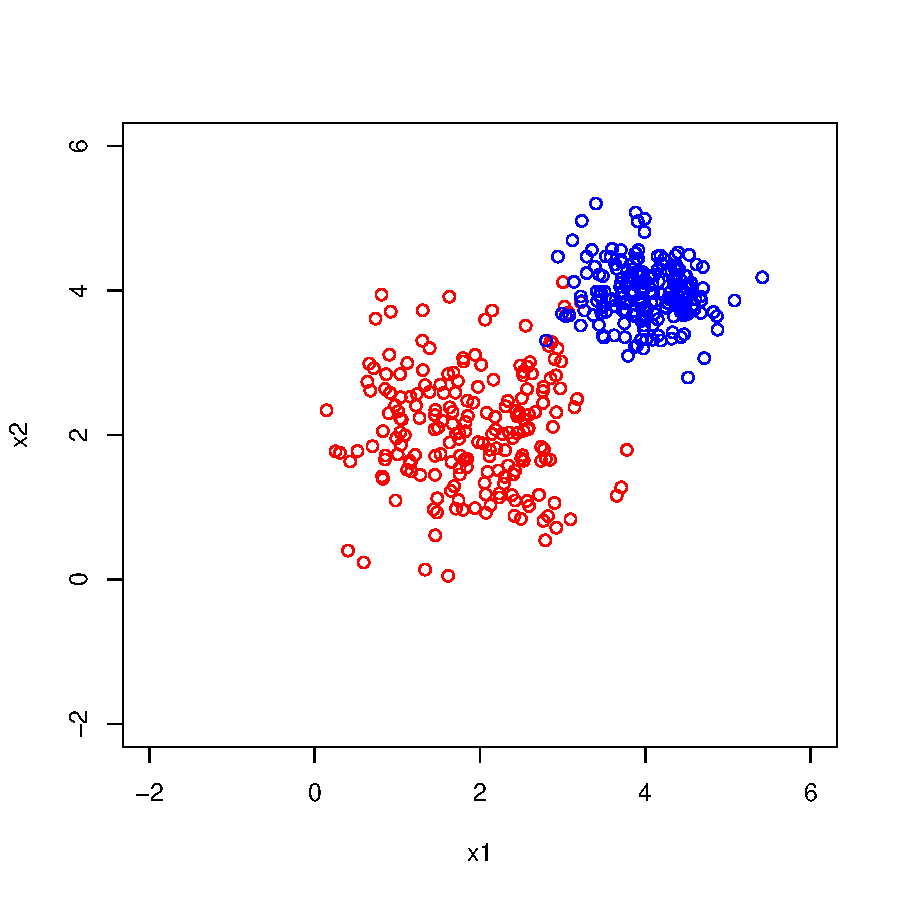
\includegraphics{BayesClassifier-004}
\caption{Dados amostrados de duas distribuições Normais com médias $m1 = (2; 2)^T$
e $m2 = (4; 4)^T$ e coeficiente de correlação nulo.}
\label{ex1}
\end{figure}

  \par Uma vez definido as amostras, iremos separar $90\%$ para construir o modelo e $10\%$ para treinar o modelo. 
  
\begin{Schunk}
\begin{Sinput}
> x <- rbind(c1, c2)
> index <- sample(1:nrow(x), length(1:nrow(x)))
> x <- x[index,]
> training_sample_number = round(nrow(x)*0.9)
> x_train <- x[1:training_sample_number,]
> x_test <- x[(training_sample_number+1):nrow(x), ]
> bayes_classifier(x_train, x_test)
\end{Sinput}
\begin{Soutput}
 [1] 0 0 0 1 0 0 1 1 0 1 0 1 1 1 0 1 1 0 0 0 0 1 0 1 0 0 1 1 1 0 1 1 1 0 1 1 0 1
[39] 1 0
\end{Soutput}
\end{Schunk}


\section{Resultados}


\section{Conclusão}


%%%%%%%%%%%%%%%%%%%%%%%%%%%%%%%%%%%%%%%%%%%%%%%%%%%%%%%%%%%%%%%%%%%%%%%%%%%%%%%%%%%%%%%%%

%%%%%%%%%%%%%%%%%%%%%%%%%%%%%%%%%%%%%%%%%%%%%%%%%%%%%%%%%%%%%%%%%%%%%%%%%%%%%%%%%%%%%%%%%


\begin{thebibliography}{99}
		\bibitem{c1}\label{BreastCancer}
\end{thebibliography}	


\end{document}
